\documentclass{article}
\usepackage{listings}
\usepackage{graphicx}
\usepackage{amsmath}
\usepackage{amssymb}
\usepackage{color}
\usepackage{float}
\usepackage{geometry}
\usepackage{tikz}
\usepackage{url}
\usepackage{lettrine}
\lstset{
    basicstyle = \sffamily,
    keywordstyle = \bfseries,
    commentstyle = \rmfamily\itshape,
    stringstyle = \ttfamily,
    flexiblecolumns,
    numbers = left,
    showspaces = false,
    numberstyle = \ttfamily,
    showstringspaces = false,
    captionpos = t,
    frame = lrtb,
}
\lstdefinestyle{Python}{
    language = Python,
    basicstyle = \ttfamily,
    numberstyle = \ttfamily,
    keywordstyle = \color{blue},
    keywordstyle = [2] \color{teal},
    stringstyle = \color{magenta},
    commentstyle = \color{red}\ttfamily,
    breaklines = true,
    columns = fixed,
    basewidth = 0.5em,
}
\usepackage[framemethod=tikz]{mdframed}

\title{Localization System of Group A2}
\author{Wu Chengyu\ \url{7086cmd@gmail.com}}
\date{\today}

\begin{document}
\maketitle

\newpage

\tableofcontents

\newpage

\section{Introduction}

\lettrine{T}{he} map of the contest is a 2D plane with \texttt{apriltags} on it. The \texttt{apriltags} are asymmetrical and easy to recognize.

Through the camera, we can fetch all the \texttt{apriltags} in the view of the camera. Using \texttt{OpenCV}, we can get the position of the \texttt{apriltags} in the image. Then we can use the position of the \texttt{apriltags} to calculate the position of the camera.

The \texttt{ROS} (Robot Operating System) provides apis to get the position of the \texttt{apriltags} in the image. However, we also need the camera to recognize other blocks, e.g. the ``fish'' in the contest. So we deprecated the \texttt{ROS} and simply use \texttt{Python} with \texttt{OpenCV} to get the position of the \texttt{apriltags} in order to locate.

Also, we need to recognize blocks colored with red, yellow, green, and blue (size: $5\mathrm{cm}\times5\mathrm{cm}\times5\mathrm{cm}$). We should use \texttt{OpenCV} too, so it's a good manner to combine these two parts together.

That's the biggest reason why I strongly recommend navigating with \texttt{OpenCV}.

Becuase we don't use \texttt{ROS}, so we can test the camera with my laptop. The Apple 1080P camera can help me to test the algorithm. As for the calculation difference, it is not so big.

\section{Targets}

There are several targets in this project:

\subsection{Calibration}

\begin{itemize}
  \item Get the camera matrix and the distortion coefficients with the help of \texttt{OpenCV}.
  \item Store the data, and use it at call time.
  \item Fetch the external parameters when the robot is on a apriltag and calculate the transform matrixes to get the external parameters.
\end{itemize}

\subsection{Localization \& Navigation}

\textbf{NOTE: Finally, this plan is deprecated.}

\begin{itemize}
  \item We need fetch the location of the robot (not only position, but also the orientation) in the ground coordinate system. The ground coordinate system is defined by the \texttt{apriltags}.
  \item We need to adjust the position, making it more accurate. The accuracy should be less than $1\mathrm{cm}$.
  \item We need to handle with the emergency situation. If there are less than $3$ \texttt{apriltags} in the view of the camera, we should use corner of single \& double \texttt{apriltags} to calculate the position of the camera.
  \item If there is no \texttt{apriltags} in the view of the camera, we should turn around and find the \texttt{apriltags}.
\end{itemize}

\textbf{NOTE: The Current Plan}

We use the \texttt{apriltags} with its 4 corners to calculate the position of the camera. We use the P$n$P algorithm to calculate the position of the camera.

So, in general, even if there is only one \texttt{apriltag} in the view of the camera, we can calculate the position of the camera.

\subsection{Block Recognition}

\begin{itemize}
  \item We need to recognize the color of the block. The color of the block is red, yellow, green, and blue. If necessary, we need to recognize the orange block too.
  \item We should get the camera matrix, the distortion coefficients. However, it's not my task.
  \item We should also get the position of the block (only position) in the ground coordinate system.
\end{itemize}

\subsection{Interprocess Communication}

The \texttt{CV} is a independent module, and it should communicate with the control kernel. We should use the \texttt{socket.io} to communicate between the \texttt{CV} and the control kernel.

\section{Project Structure (CV)}

The project is a \texttt{Python} project with modules. It relys on \texttt{OpenCV}, \texttt{numpy}, \texttt{pupil\_apriltag}, and \texttt{python-socketio}.

The project structure is as follows:

\begin{itemize}
  \item \texttt{calibration}: The calibration methods, including \texttt{external} and \texttt{internal} calibration.
  \item \texttt{localization}: The localization that can calculate the position of the camera and the vehicle in the ground coordinate system.
  \item \texttt{recognition}: The recognition can calculate the position of the block in the ground coordinate system with the help of the \texttt{localization} module.
  \item \texttt{configuration}: The data configuration of \texttt{colors} (color range of the block) and \texttt{tags} (the position of the \texttt{apriltags} in the ground coordinate system).
  \item \texttt{main.py}: The main file of the project. It contains the main function, and is responsible for the communication between the \texttt{CV} and the control kernel.
\end{itemize}

\section{Methodological Analysis}
In general, positioning requires $6$ degrees of freedom. That is to say, we need at least $6$ points to calculate the accurate position of the camera. However, the $3$ degrees of freedom will remain constant during the robot's motion.

For spatial coordinates, we use the Cartesian coordinate system $\left(x,y,z\right)$. For the angular coordinates, we use the Euler angle $\left(\alpha,\beta,\gamma\right)$. Or we can call it $\left(\mathrm{roll},\mathrm{pitch},\mathrm{yaw}\right)$.

The punctuation of \texttt{apriltags} is fixed, therefore, as long as we know the position of \texttt{apriltags} in the image and its punctuation, it is possible to correspond the two-dimensional image coordinates to the three-dimensional spatial coordinates. Using P$n$P algorithm, we can get the position of the camera.

\subsection{Calibration}

The calibration is divided into $2$ parts: \texttt{external} and \texttt{internal} calibration.

The first step is the \texttt{internal} calibration, which is to get the camera matrix and the distortion coefficients. We should use a chess board to get the camera matrix and the distortion coefficients, with different angles and distances.

The internal calibration process is quite simple. We can use the \texttt{calibrateCamera} method provided by \texttt{OpenCV} to get the camera matrix and the distortion coefficients.

For fun, I provided a simple internal parameter calibration method that can calibrate the camera promptly with the camera. You may turn around to get the accurate calibration data. That's quite fun, or funny.

Then, we should put our robot on a \texttt{apriltag}. Of course, you can put the robot anywhere since you know the position of the robot and the camera (using the P$n$P algorithm is more preferable). Then, we can calculate the transform matrix with the help of the ground coordinate system.

As we know, the transform of $2$ coordinate systems is a $4\times4$ matrix. You can describe it as:

\begin{equation}
  \boldsymbol{T} (\texttt{homogeneous\_matrix})=\left(
    \begin{matrix}
      \boldsymbol{R}_{ct} & \boldsymbol{t}_{ct} \\
      \boldsymbol{0} & 1
    \end{matrix}
  \right)
\end{equation}

And the procedure is (e. g. from \texttt{camera} to \texttt{vehicle}):
\begin{equation}
  \left(
    \begin{matrix}
      x_v \\
      y_v \\
      z_v \\
      1
    \end{matrix}
  \right)=\left(
    \begin{matrix}
      \boldsymbol{R}_{ct} & \boldsymbol{t}_{ct} \\
      \boldsymbol{0} & 1
    \end{matrix}
  \right)\cdot\left(
    \begin{matrix}
      x_c \\
      y_c \\
      z_c \\
      1
    \end{matrix}
  \right)
\end{equation}

\subsubsection{Mathmetical Model}

If you think this part is too boring, you can skip it, or you can take a break and tear up this article.

\paragraph{Transform Relationships}

We can get the transform matrix through the \texttt{camera} -- \texttt{world} and the \texttt{world} -- \texttt{vehicle} transform matrixes.

Then, the transform matrix from \texttt{camera} to \texttt{vehicle} is:

\begin{equation}
  \boldsymbol{T}_{cv}=\boldsymbol{T}_{cw}\cdot\boldsymbol{T}_{wv}
\end{equation}

The procedure is following:

\begin{enumerate}
  \item Through the P$n$P algorithm (\texttt{resolvePnP} in \texttt{OpenCV}), we can get the transform matrix from \texttt{world} to \texttt{camera}:
  \begin{equation}
    \left(
      \begin{matrix}
        x_c \\
        y_c \\
        z_c \\
        1
      \end{matrix}
    \right) = \left(\begin{matrix}\boldsymbol{R}_{wc} & \boldsymbol{t}_{wc} \\
        \boldsymbol{0} & 1\end{matrix}\right)\cdot\left(
        \begin{matrix}
          x_w \\
          y_w \\
          z_w \\
          1
        \end{matrix}
    \right)
  \end{equation}
  \item Then, we can use the vector $\left(\begin{matrix}1 & 0 & 0\end{matrix}\right)$ to get the transform matrix from \texttt{world} to \texttt{vehicle}, and the rotate matrix is a $3\times3$ unit matrix:

  \textbf{Note:} You must confirm that your robot's orientation is the same as the $x$-axis of the ground coordinate system. If not, you should adjust the orientation of the robot to make it the same as the $x$-axis of the ground coordinate system.

  That's because when calibrating, there is no way to get the orientation of the robot. Also, the calculation of the orientation is not so accurate. So, we should adjust the orientation of the robot to make it the same as the $x$-axis of the ground coordinate system. That's more accurate and convenient.

  So, the rotate matrix is a $3\times3$ unit matrix $\left(\begin{matrix}1&0&0\\0&1&0\\0&0&1\end{matrix}\right)$, and the position in the vehicle coordinate system is $\left(0,0,0\right)$. That's because it's the origin of the vehicle coordinate system.

  After getting the $x, y$ coordinate in the world coordinate system, and because the \texttt{apriltags} are on the ground, we can easily get $2$ transform vectors:

  \begin{equation}
    \boldsymbol{t}_{w} = \left(\begin{matrix}x_w&y_w&0\end{matrix}\right), \boldsymbol{t}_{v} = \left(\begin{matrix}0&0&0\end{matrix}\right)
  \end{equation}

  So, the \texttt{tvecs} (transform vector) is $\boldsymbol{t}_{w} - \boldsymbol{t}_{v}$. The rotate matrix is a $3\times3$ unit matrix.

  Then, we use \texttt{vstack} and \texttt{hstack} to get the full transform matrix.

  \textbf{Note:} The result of \texttt{solvePnP} is the rotate vector and the transform vector. We can use the \texttt{Rodrigues} method to get the rotate matrix.

  \item Then, we can replace the matrix $\left(\begin{matrix}x_w\\y_w\\z_w\\1\end{matrix}\right)$ with the matrix $\boldsymbol{T}_{cw}\cdot\left(\begin{matrix}x_c\\y_c\\z_c\\1\end{matrix}\right)$ to get the transform matrix from \texttt{camera} to \texttt{vehicle}:

  \begin{equation}
    \boldsymbol{T}_{cw}\cdot\left(\begin{matrix}x_c\\y_c\\z_c\\1\end{matrix}\right) = \boldsymbol{T}_{vw}\cdot\boldsymbol{T}_{cv}\cdot\left(\begin{matrix}x_c\\y_c\\z_c\\1\end{matrix}\right)
  \end{equation}

  Because the vectors in the left and right are the same, we can get relationships between these matrixes:

  \begin{equation}
    \boldsymbol{T}_{cw} = \boldsymbol{T}_{vw}\cdot\boldsymbol{T}_{cv}
  \end{equation}

  So, we can get the transform matrix from \texttt{camera} to \texttt{vehicle} through the transform matrix from \texttt{world} to \texttt{vehicle} and the transform matrix from \texttt{world} to \texttt{camera}:

  \begin{equation}
    \boldsymbol{T}_{cv} = \boldsymbol{T}^{-1}_{vw}\cdot\boldsymbol{T}_{cw} = \boldsymbol{T}_{wv}\cdot\boldsymbol{T}_{cw}
  \end{equation}

  \item Then, we can use \texttt{numpy.linalg.inv} to get the inverse matrix of $\boldsymbol{T}_{vw}$, and then dot it with $\boldsymbol{T}_{cw}$ to get the transform matrix from \texttt{camera} to \texttt{vehicle}.
\end{enumerate}

That's quite simple, isn't it?

\subsubsection{Basic Parameters}
We need the camera's internal reference and distortion coefficients to accurately confirm the conversion.

The camera's internal reference is a $3\times3$ matrix, which is the camera's focal length and the center of the image:

\[
  \texttt{camera\_matrix}=\left(\begin{matrix}
    f_x & 0 & c_x \\
    0 & f_y & c_y \\
    0 & 0 & 1
  \end{matrix}\right)
\]

The distortion coefficients are $5$ parameters, which are used to correct the distortion of the image:

\[
  \texttt{distortion\_coefficients}=\left(\begin{matrix}
    k_1 & k_2 & p_1 & p_2 & k_3
  \end{matrix}\right)
\]

The relevant parameters of the camera are not considered to vary excessively during the process. In other words, we can store these parameters directly at call time.

\subsection{Localization}

\begin{mdframed}
  \textbf{Note:} These methods are deprecated. We import the \texttt{apriltags}'s corners (range: left -- up, right -- up, right -- down, left -- down). Through the range and the width of the tag in the ground tag, we can get $4$ or $5$ points to calculate points.
\end{mdframed}

\subsubsection{6-point Adjustment}
Each location of the \texttt{apriltags} can define $\dfrac16$ of the camera's position. Therefore, we need at least $6$ \texttt{apriltags} to calculate the position of the camera.

\[
  \left(
    \begin{matrix}
      x&y&z\\
      \mathrm{roll}&\mathrm{pitch}&\mathrm{yaw}
    \end{matrix}
  \right)
\]

Through the P$n$P algorithm provided by \texttt{OpenCV}, we can calculate the transform vector and the rotation vector of the camera easily.

After getting \texttt{tvec} and \texttt{rvec}, we can use the \texttt{Rodrigues} function to convert the rotation vector to the rotation matrix:

\[
  \boldsymbol{R}\_\texttt{mtx}=\texttt{Rodrigues}\left(\texttt{rvec}\right)
\]

Then, through some simple calculations, we can get the Euler angle.

\subsubsection{3-point Localization}
The \texttt{apriltags}'s center point is accurate enough to calculate the position of the camera. That is to say, through at least $3$ \texttt{apriltags}, we can calculate the position of the camera through the P$n$P algorithm.

Knowing $z$, $\mathrm{roll}$ and $\mathrm{pitch}$, we should calculate the ``bias'' matrix.

Define the original matrixes of rotate and transform through these elements:

\begin{equation}
  \boldsymbol{R}_x=
  \left(
    \begin{matrix}
      1 & 0 & 0 \\
      0 & \cos\alpha & -\sin\alpha \\
      0 & \sin\alpha & \cos\alpha
    \end{matrix}
  \right),
  \boldsymbol{R}_y=
  \left(
    \begin{matrix}
      \cos\beta & 0 & \sin\beta \\
      0 & 1 & 0 \\
      -\sin\beta & 0 & \cos\beta
    \end{matrix}
  \right)
\end{equation}

Then, we can get the rotate ``bias'' matrix:

\begin{equation}
  \boldsymbol{R}_{\texttt{bias}}=\boldsymbol{R}_x\cdot \boldsymbol{R}_y= \left(
    \begin{matrix}
      \cos\beta & 0 & \sin\beta \\
      \sin\alpha\sin\beta & \cos\alpha & -\sin\alpha\cos\beta \\
      -\cos\alpha\sin\beta & \sin\alpha & \cos\alpha\cos\beta
    \end{matrix}
  \right)
\end{equation}

Through \texttt{Rodrigues} method, we can get the rotate vector of the ``bias'' matrix.

Also, the transform vector is easy to get:

\begin{equation}
  \boldsymbol{t}_{\texttt{bias}}=\left(
    \begin{matrix}
      0 \\
      0 \\
      -z
    \end{matrix}
  \right)
\end{equation}

\subsubsection{1-point Emergency Localization}
We can know each corner of the \texttt{apriltags} of the map. Therefore, we can calculate the position of the camera through the P$n$P algorithm.

However, I strongly recommend that we should not use this method. It is not so accurate and it is easy to make mistakes.

If there is less than $3$ \texttt{apriltags} in the view of the camera, we can calculate corners of the \texttt{apriltags} in the image. Then we can calculate the position of the camera through the P$n$P algorithm.

\subsubsection{Turn Around}
The robot can never gonna give you up, never gonna let you down. It can never gonna run around and desert you.

So, don't cry, don't say goodbye, don't tell a lie and hurt you.

If there's no \texttt{apriltags}, what the robot should do is to turn around and find the \texttt{apriltags}. There is no place without \texttt{apriltag} around the robot.

\subsubsection{Used Algorithm}

In order to calculate the position of the vehicle (using the \texttt{external parameters}), we can use the multiplication of the \texttt{world} -- \texttt{camera} (P$n$P) and the \texttt{camera} -- \texttt{vehicle} (external parameter) transform matrixes to get the \texttt{vehicle} -- \texttt{world} transform matrix.

We finally decided to deprecate the Eular Angle and use the Heading Angle instead. I selected the $x$-axis of the ground coordinate system as the $0^\circ$ angle, and it is actually the \texttt{yaw}.

Then, in order to improve the accurate, I decided to use corners and centers together. Although the $1, 3, 6$ method was deprecated, its idea is still useful. What it inspired me is one point can decide one free degree in average.

\subsection{Block Recognition}

\subsubsection{Color Recognition}
Through the \texttt{HSV} color space, we can easily recognize the color of the block. The \texttt{HSV} color space is a cylindrical coordinate system. The three dimensions represent the hue, saturation, and value, respectively.

We use the opening operation to remove the noise. That's becuase there are white dots on colored blocks and it is not so easy to remove. The opening operation can relatively remove the white dots, making the color recognition more accurate.

The adjustment of target range is a hard work. We should adjust the range of the color recognition to make it more accurate.

\subsubsection{Shape Recognition}

\paragraph{Recognition}

Due to the interference of the points in the dice, we cannot determine the outline of each dice very accurately. But the closer the distance, the higher the definition.

We use \texttt{HSV} color space to recognize the color of the dice. Before recognizing, we use the opening operation to remove some noise. You can see the action in the next section.

Then, we calculated the transform matrix, and use the \texttt{warpPerspective} function to transform the image:

\begin{equation}
  \boldsymbol{R}_x=
  \left(
  \begin{matrix}
    1 & 0 & 0 \\
    0 & \cos\theta & -\sin\theta \\
    0 & \sin\theta & \cos\theta
  \end{matrix}
  \right),
  \boldsymbol{R}_y=
  \left(
  \begin{matrix}
    \cos\phi & 0 & \sin\phi \\
    0 & 1 & 0 \\
    -\sin\phi & 0 & \cos\phi
  \end{matrix}
  \right),
  \boldsymbol{R}_z=
  \left(
  \begin{matrix}
    \cos\psi & -\sin\psi & 0 \\
    \sin\psi & \cos\psi & 0 \\
    0 & 0 & 1
  \end{matrix}
  \right)
\end{equation}

It is the rotate matrix from Eular Angle.

Then, we firstly dot the $\boldsymbol{R}_x$ and $\boldsymbol{R}_y$ matrixes, and then dot the result with $\boldsymbol{R}_z$ matrix. We can get the transform matrix.

\begin{equation}
  \boldsymbol{R}_{\texttt{transform}}=\boldsymbol{R}_z\cdot\left(\boldsymbol{R}_x\cdot\boldsymbol{R}_y\right)
\end{equation}

The vertical transform vector is quite easy. Just simply resize it.

Then, we can get the full matrix through \texttt{hstack} and \texttt{vstack} method. You can see the full algorithm in next section.

\paragraph{Calculation}

The camera can only capture the two-dimensional image. So we simply use the \texttt{N2} algorithm to abstract objects into particles:

\[
  \left(\begin{matrix}x&y\end{matrix}\right)=\left(\begin{matrix}\sqrt{\dfrac{\sum x_i^2}{n}}&\sqrt{\dfrac{\sum y_i^2}{n}}\end{matrix}\right)
\]

The reason why the arithmetic mean is not used is because I think it is not elegant enough.

\subsection{Communicating}

Because the version supportation problems, we finally decide to use \texttt{socket.io} to communicate between the contorl kernel and the vision module. The \texttt{python-socketio} provides the full package, and we can easily realize it.

The communication can be described as only the \texttt{send-to-receive} procedure. The CV core sends the location data, and the control core (maybe \texttt{ROS}) receive it and send it to the computing program to calculate the best way.

\section{Algorithm Implementation}

Using P$n$P method, we can get the location of the camera easily. The project structure includes \texttt{localization} folder, and it is the core of the localization module.

\subsection{Kernel: class \texttt{Location}}

I packed the method into the class \texttt{Location}. It contains position, orientation (Euler angle), the camera matrix and the distortion coefficients which is saved in \texttt{data/calibration.npz}.

The \texttt{x}, \texttt{y}, \texttt{z}, \texttt{roll}, \texttt{pitch}, \texttt{yaw} are the position and orientation of the camera. The \texttt{camera\_matrix} and \texttt{distortion\_coefficients} are the camera matrix and the distortion coefficients.

\texttt{x}, \texttt{y}, \texttt{z}, \texttt{roll}, \texttt{pitch}, \texttt{yaw} are \texttt{np.float32} type, and the \texttt{camera\_matrix} is a $3\times3$ \texttt{np.ndarray} matrix with \texttt{np.float32}, and the \texttt{distortion\_coefficients} is a $5\times1$ \texttt{np.ndarray} matrix with \texttt{np.float32}.

The kernel will detect \texttt{data/calibration.npz} file, if there's no parameters or the file is not exist, it will raise an error.

\textbf{Note} Because the author is familiar with \texttt{HTTP Methods}, the introduction of classes and methods is written in ``the form of \texttt{HTTP Methods}''.

\subsubsection{\texttt{POST} Methods -- Initialization}

You need to initialize the class \texttt{Location} with the \texttt{camera\_matrix} and the \texttt{distortion\_coefficients}. If you don't want to directly write the parameters, you can use the \texttt{calibrate} method to calibrate the camera. If there's no parameters, the initialization method will read the parameters from \texttt{data/calibration.npz}.

If there's still no parameters, the initialization method will raise an error: \texttt{Calibration file does not exist}.


\subsubsection{\texttt{GET} Methods}

The \texttt{Location} class provides variety of methods to return the position and orientation of the camera. I don't want to introduce these parameters to you, as I think you are clever enough to know them. Otherwize, you are not suitable to read this document. The methods are:

\begin{itemize}
  \item \texttt{is\_adjusted}: Return \texttt{True} if the camera is adjusted, otherwise return \texttt{False}.
  \item \texttt{get\_z}: Return the $z$-axis value of the camera.
  \item \texttt{get\_position}: Return the position of the camera. The return type is $\left(x,y,z\right)$.
  \item \texttt{get\_orientation}: Return the orientation of the camera. The return type is $\left(\mathrm{roll},\mathrm{pitch},\mathrm{yaw}\right)$.
  \item \texttt{get\_camera\_matrix}: Return the camera matrix:
  \[
    \texttt{camera\_matrix}=\left(\begin{matrix}
      f_x & 0 & c_x \\
      0 & f_y & c_y \\
      0 & 0 & 1
    \end{matrix}\right)
  \]
  \item \texttt{get\_distortion\_coefficients}: Return the distortion coefficients:
  \[
    \texttt{distortion\_coefficients}=\left(\begin{matrix}
      k_1 & k_2 & p_1 & p_2 & k_3
    \end{matrix}\right)
  \]
  \textbf{Note: } $2$ functions above has been stored since the initialization of the class. It won't change during the process.
  \item \texttt{get\_location\_matrix}: Return the location matrix. It is a $3\times2$ matrix. The first line is the position in the ground coordinate system, and the second line is the orientation (Euler angle).
  \[
    \texttt{location\_matrix}=\left(\begin{matrix}
      x & y & z \\
      \mathrm{roll} & \mathrm{pitch} & \mathrm{yaw}
    \end{matrix}\right)
  \]
  In this document, I may regard $\theta$ as the $\mathrm{roll}$, $\phi$ as the $\mathrm{pitch}$, and $\psi$ as the $\mathrm{yaw}$.
\end{itemize}

\subsubsection{\texttt{PUT} Methods -- Adjustment and Localization}

The kernel provides functions to adjust the position and orientation of the camera. Then, you can use less \texttt{apriltags} to locate the camera.

\paragraph{Adjustment}

You can use the \texttt{adjust} method to adjust the position and orientation of the camera. The class will store $z$, $\mathrm{roll}$, and the $\mathrm{pitch}$ data.

You need provide at least $6$ \texttt{apriltags} to adjust the camera. Or the class will raise an error: \texttt{At least 6 tags are required to adjust the camera}.

\paragraph{Localization}

The class will provide a packed method to locate the camera. No matter how many \texttt{apriltags} are in the view of the camera, the class will calculate the position and orientation of the camera, (except there's no \texttt{apriltags} in the view of the camera.)

The class will use the P$n$P algorithm to calculate the position and orientation of the camera. If there's no \texttt{apriltags} in the view of the camera, the class will raise an error: \texttt{No tags in the view of the camera}.

\subsection{Other Functions}

There are also some implementation functinos. They are not so important, so I won't introduce them to you.

\section{Block Recognition}

The block recognition is implemented in the \texttt{recognition} folder. The core of the block recognition is the \texttt{BlockRecognition} class.

\subsection{Kernel: class \texttt{BlockRecognition}}

It is a class that can provide methods to recognize the color and the shape of the block. The class will use the \texttt{Location} class to get the position of the camera.

The class will use the \texttt{HSV} color space to recognize the color of the block. The class will use the \texttt{N2} algorithm to decide wich point to use to calculate the position of the block.

If you call the \texttt{recognize}, the class will automatically capture a image to recognize the block. You need to provide the color range (lower, and upper) to recognize it.

After recognition, it will save color and position of the block into \texttt{blocks}. The \texttt{blocks} is a \texttt{tuple} type. You can use \texttt{get\_blocks} method to get the \texttt{blocks}.

\subsection{Recognition Method: \texttt{detect}}

The detector will use the \texttt{HSV} color space to recognize the color of the block.

\lstinputlisting[style=Python]{../src/recognition/detector.py}

\subsection{Locate Method: \texttt{locate\_block}}
The locate method provides the location of blocks in the image and the ground coordinate system. It will fetch \texttt{camera\_matrix} and \texttt{distortion\_coefficients} from the \texttt{Location} class. It will also get the camera position and orientation from the \texttt{Location} class.

Then, it will calculate the rotate \& transform matrix ($\boldsymbol{R}_{\texttt{transform}}$ and $\boldsymbol{t}_{\texttt{transform}}$) through the position and orientation of the camera. Then, it will use the \texttt{undistortPoints} method to transform the image.

It's the core of the block localization, and it's important enough to display the code here.

\lstinputlisting[style=Python]{../src/recognition/locate.py}

According to the code, it will calculate the position of the block as well.

\section{Algorithm Effect}

The algorithm is quite effective. It can recognize the color of the block and the position of the block.

\subsection{Calibration}

\includegraphics[width=0.8\textwidth]{figure/c-1.png}

According to the image, the \texttt{OpenCV} can get the camera matrix and the distortion coefficients with chess board.

Then, we can get the data in \texttt{data/calibration.npz}.

In this demo, we get the data:

\[
  \texttt{camera\_matrix}=\left(\begin{matrix}
    1503.75365 & 0.0 & 899.284676 \\
    0.0 & 1514.5398703 & 367.845474 \\
    0.0 & 0.0 & 1.0
  \end{matrix}\right)
\]
\[
  \texttt{distortion\_coefficients}=\left(\begin{matrix}
    -0.010567 & 0.302944 & -0.070295 & -0.021696 & -0.445497
  \end{matrix}\right)
\]

Because the image is not flat enough, the calibration is not so accurate. However, it is enough for the algorithm.

Then, we can see the file in \texttt{data} folder.

\subsection{Localization}

\subsubsection{AprilTag Caption}

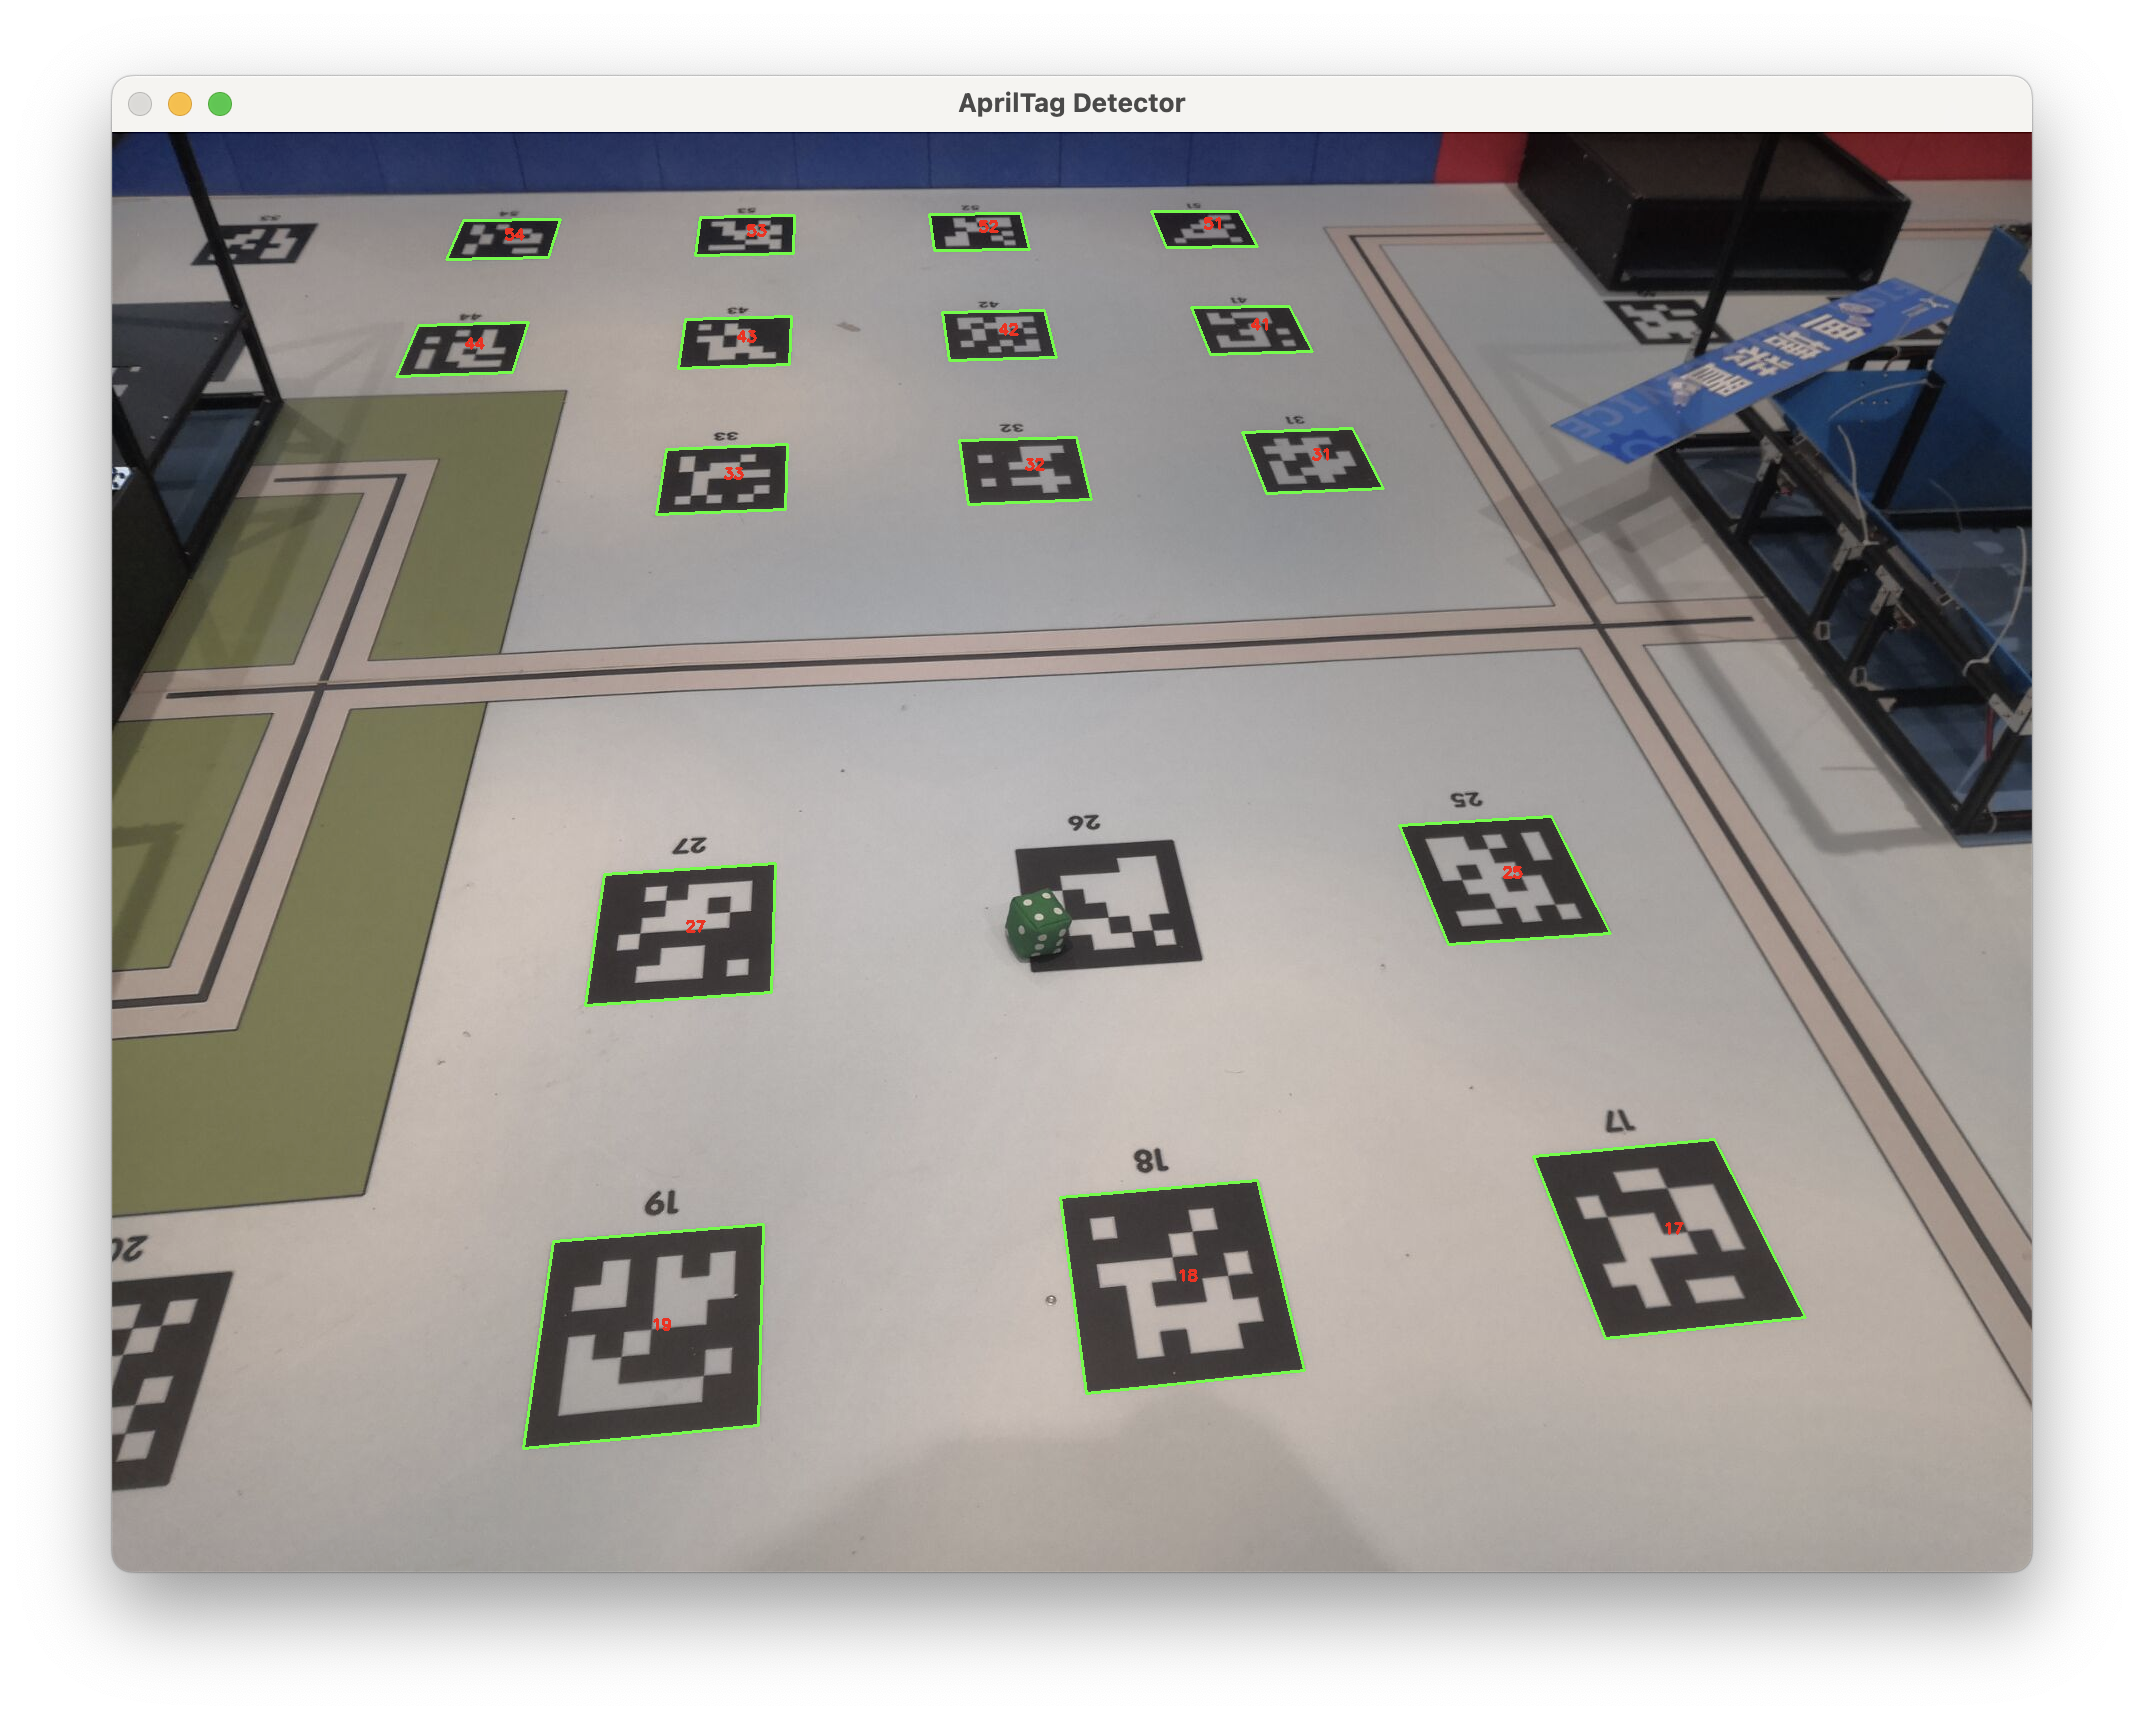
\includegraphics[width=0.8\textwidth]{figure/l-1.png}

The \texttt{OpenCV} and the \texttt{pupil\_apriltag} package can recognize \texttt{package} properly. The picture above can show the effect.

Then, through at laast $6$ \texttt{apriltags}, we can adjust the position and orientation of the camera.

For example, the position and orientation of the camera (prompt) in the following picture:

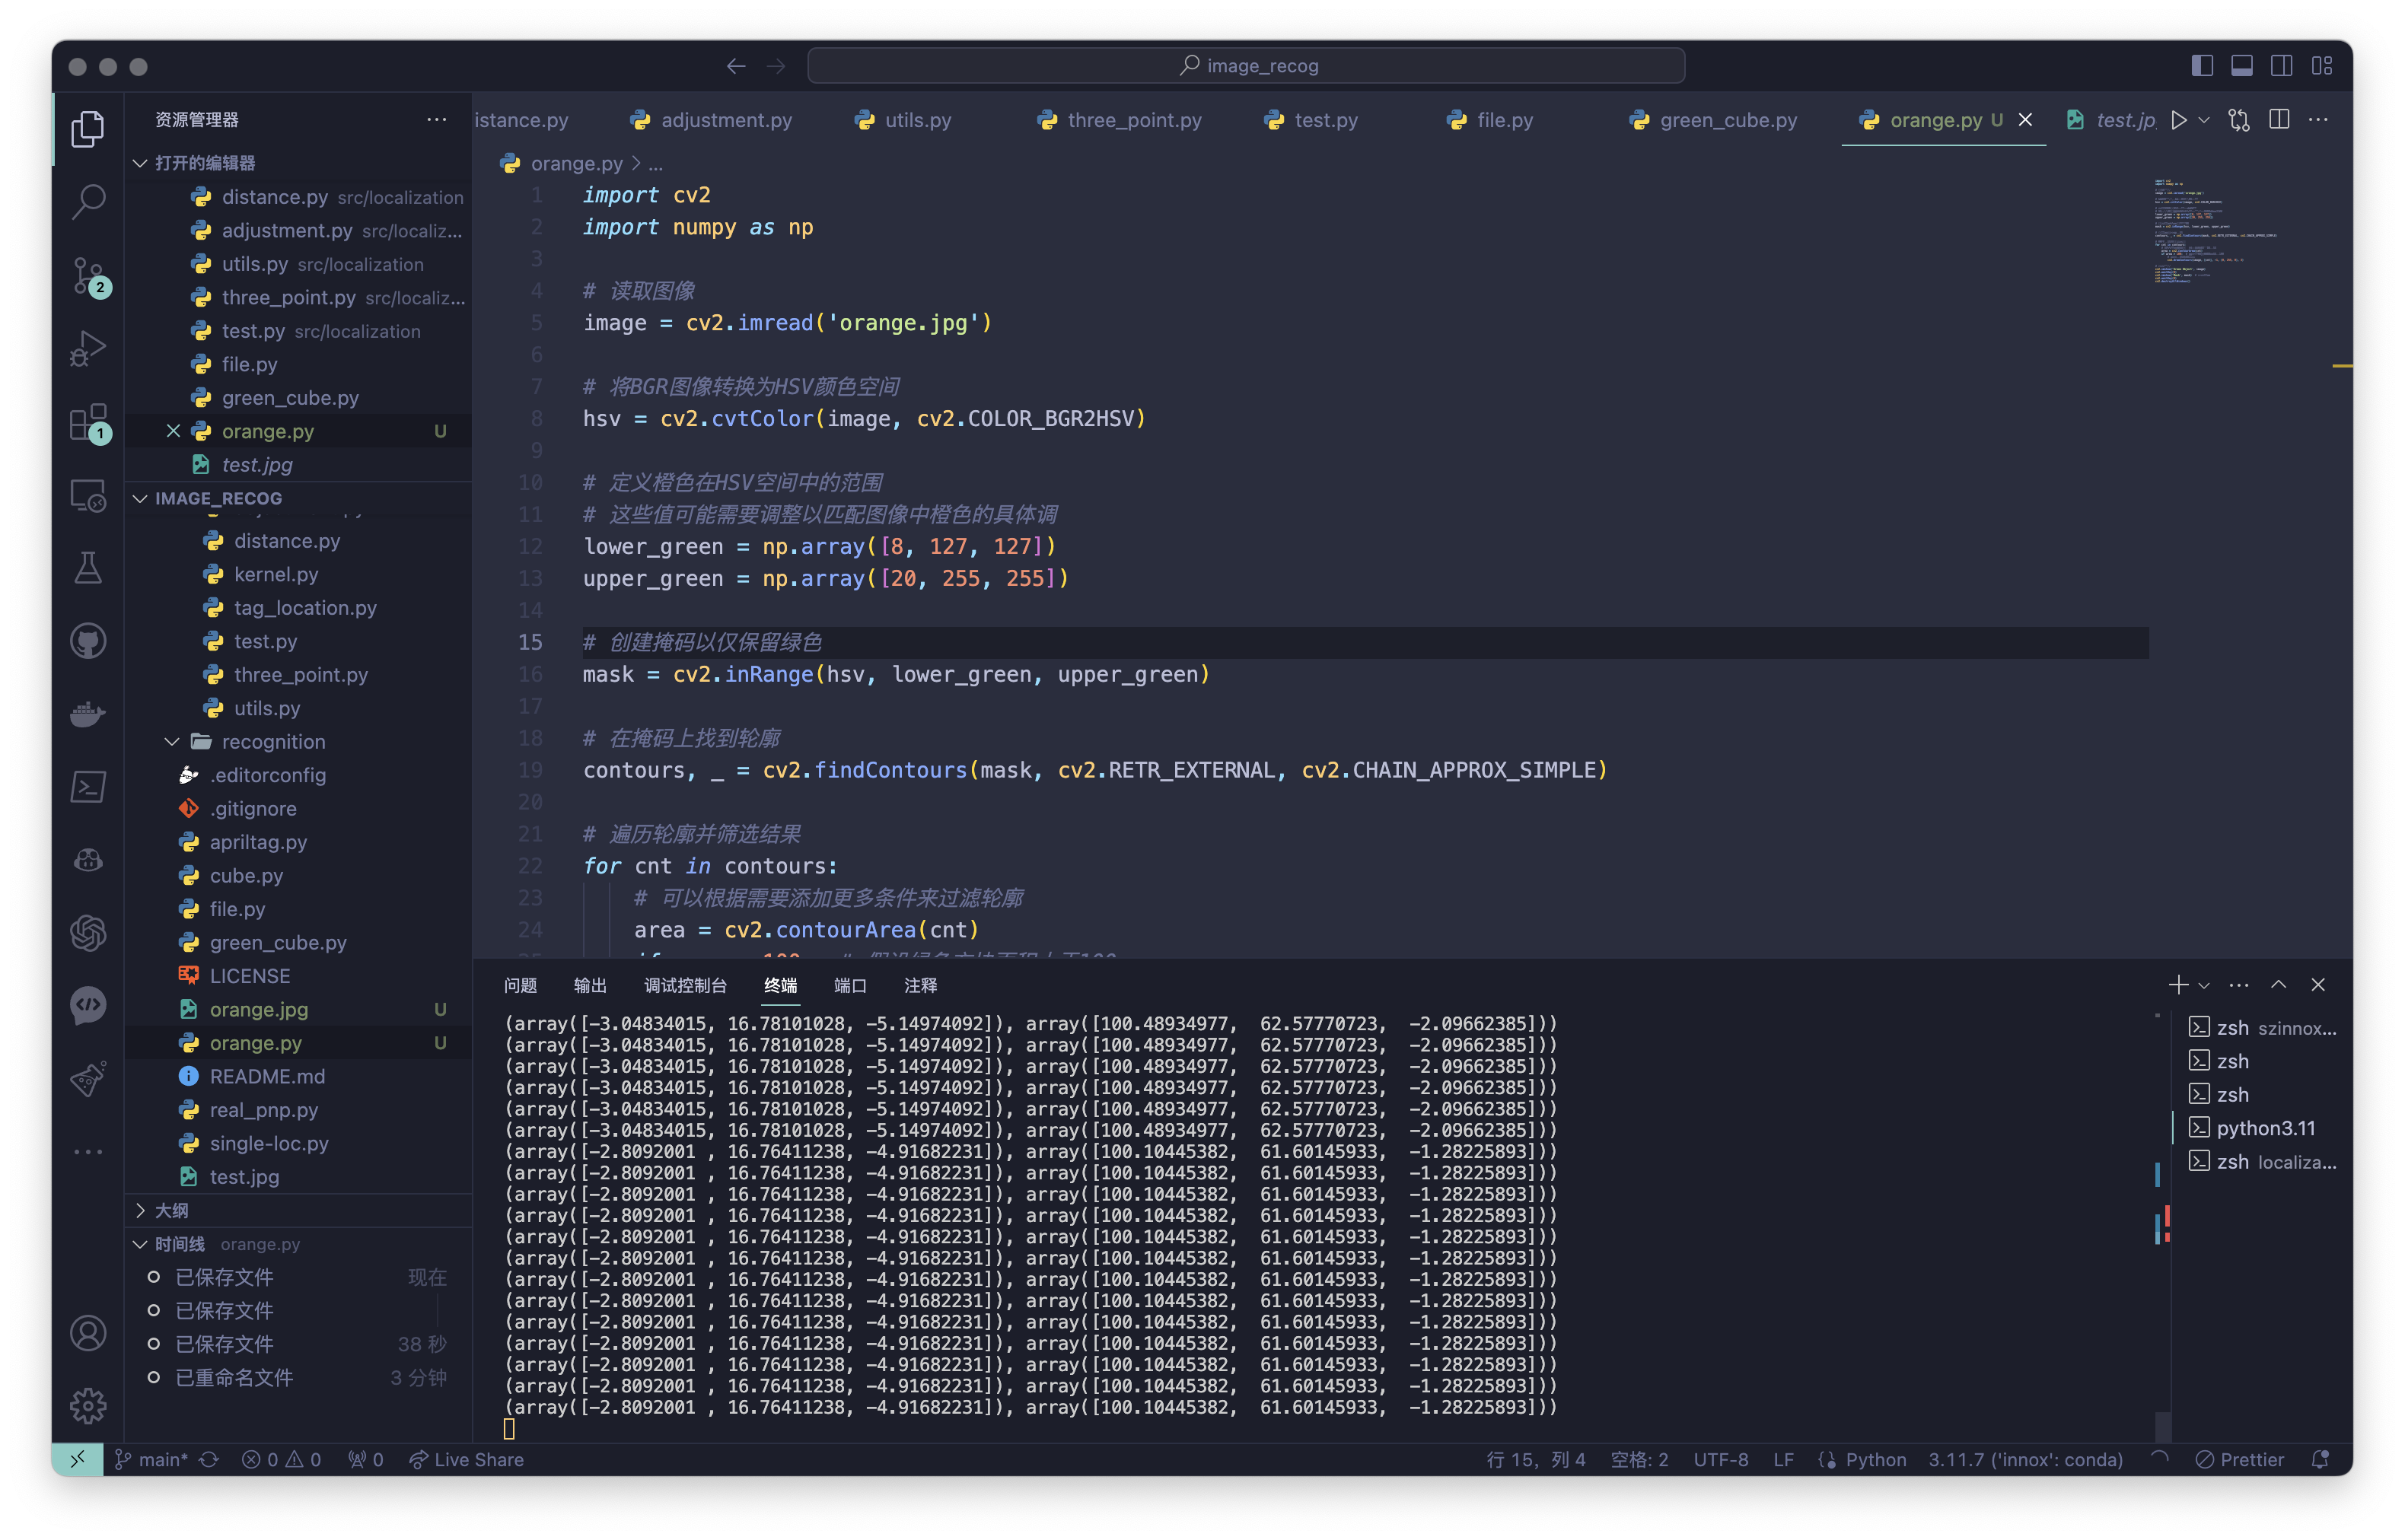
\includegraphics[width=0.8\textwidth]{figure/l-2.png}

The array is $\left(x,y,z,\mathrm{roll},\mathrm{pitch},\mathrm{yaw}\right)$.\\\indent It can display as $\left(\begin{matrix}-2.8092001&16.76411238&4.916822&100.10445382&61.60145933&-1.28225893\end{matrix}\right)$ when testing with my laptap.

\subsubsection{Block Recognition}

The color recognition can work properly. The picture above can show the effect.

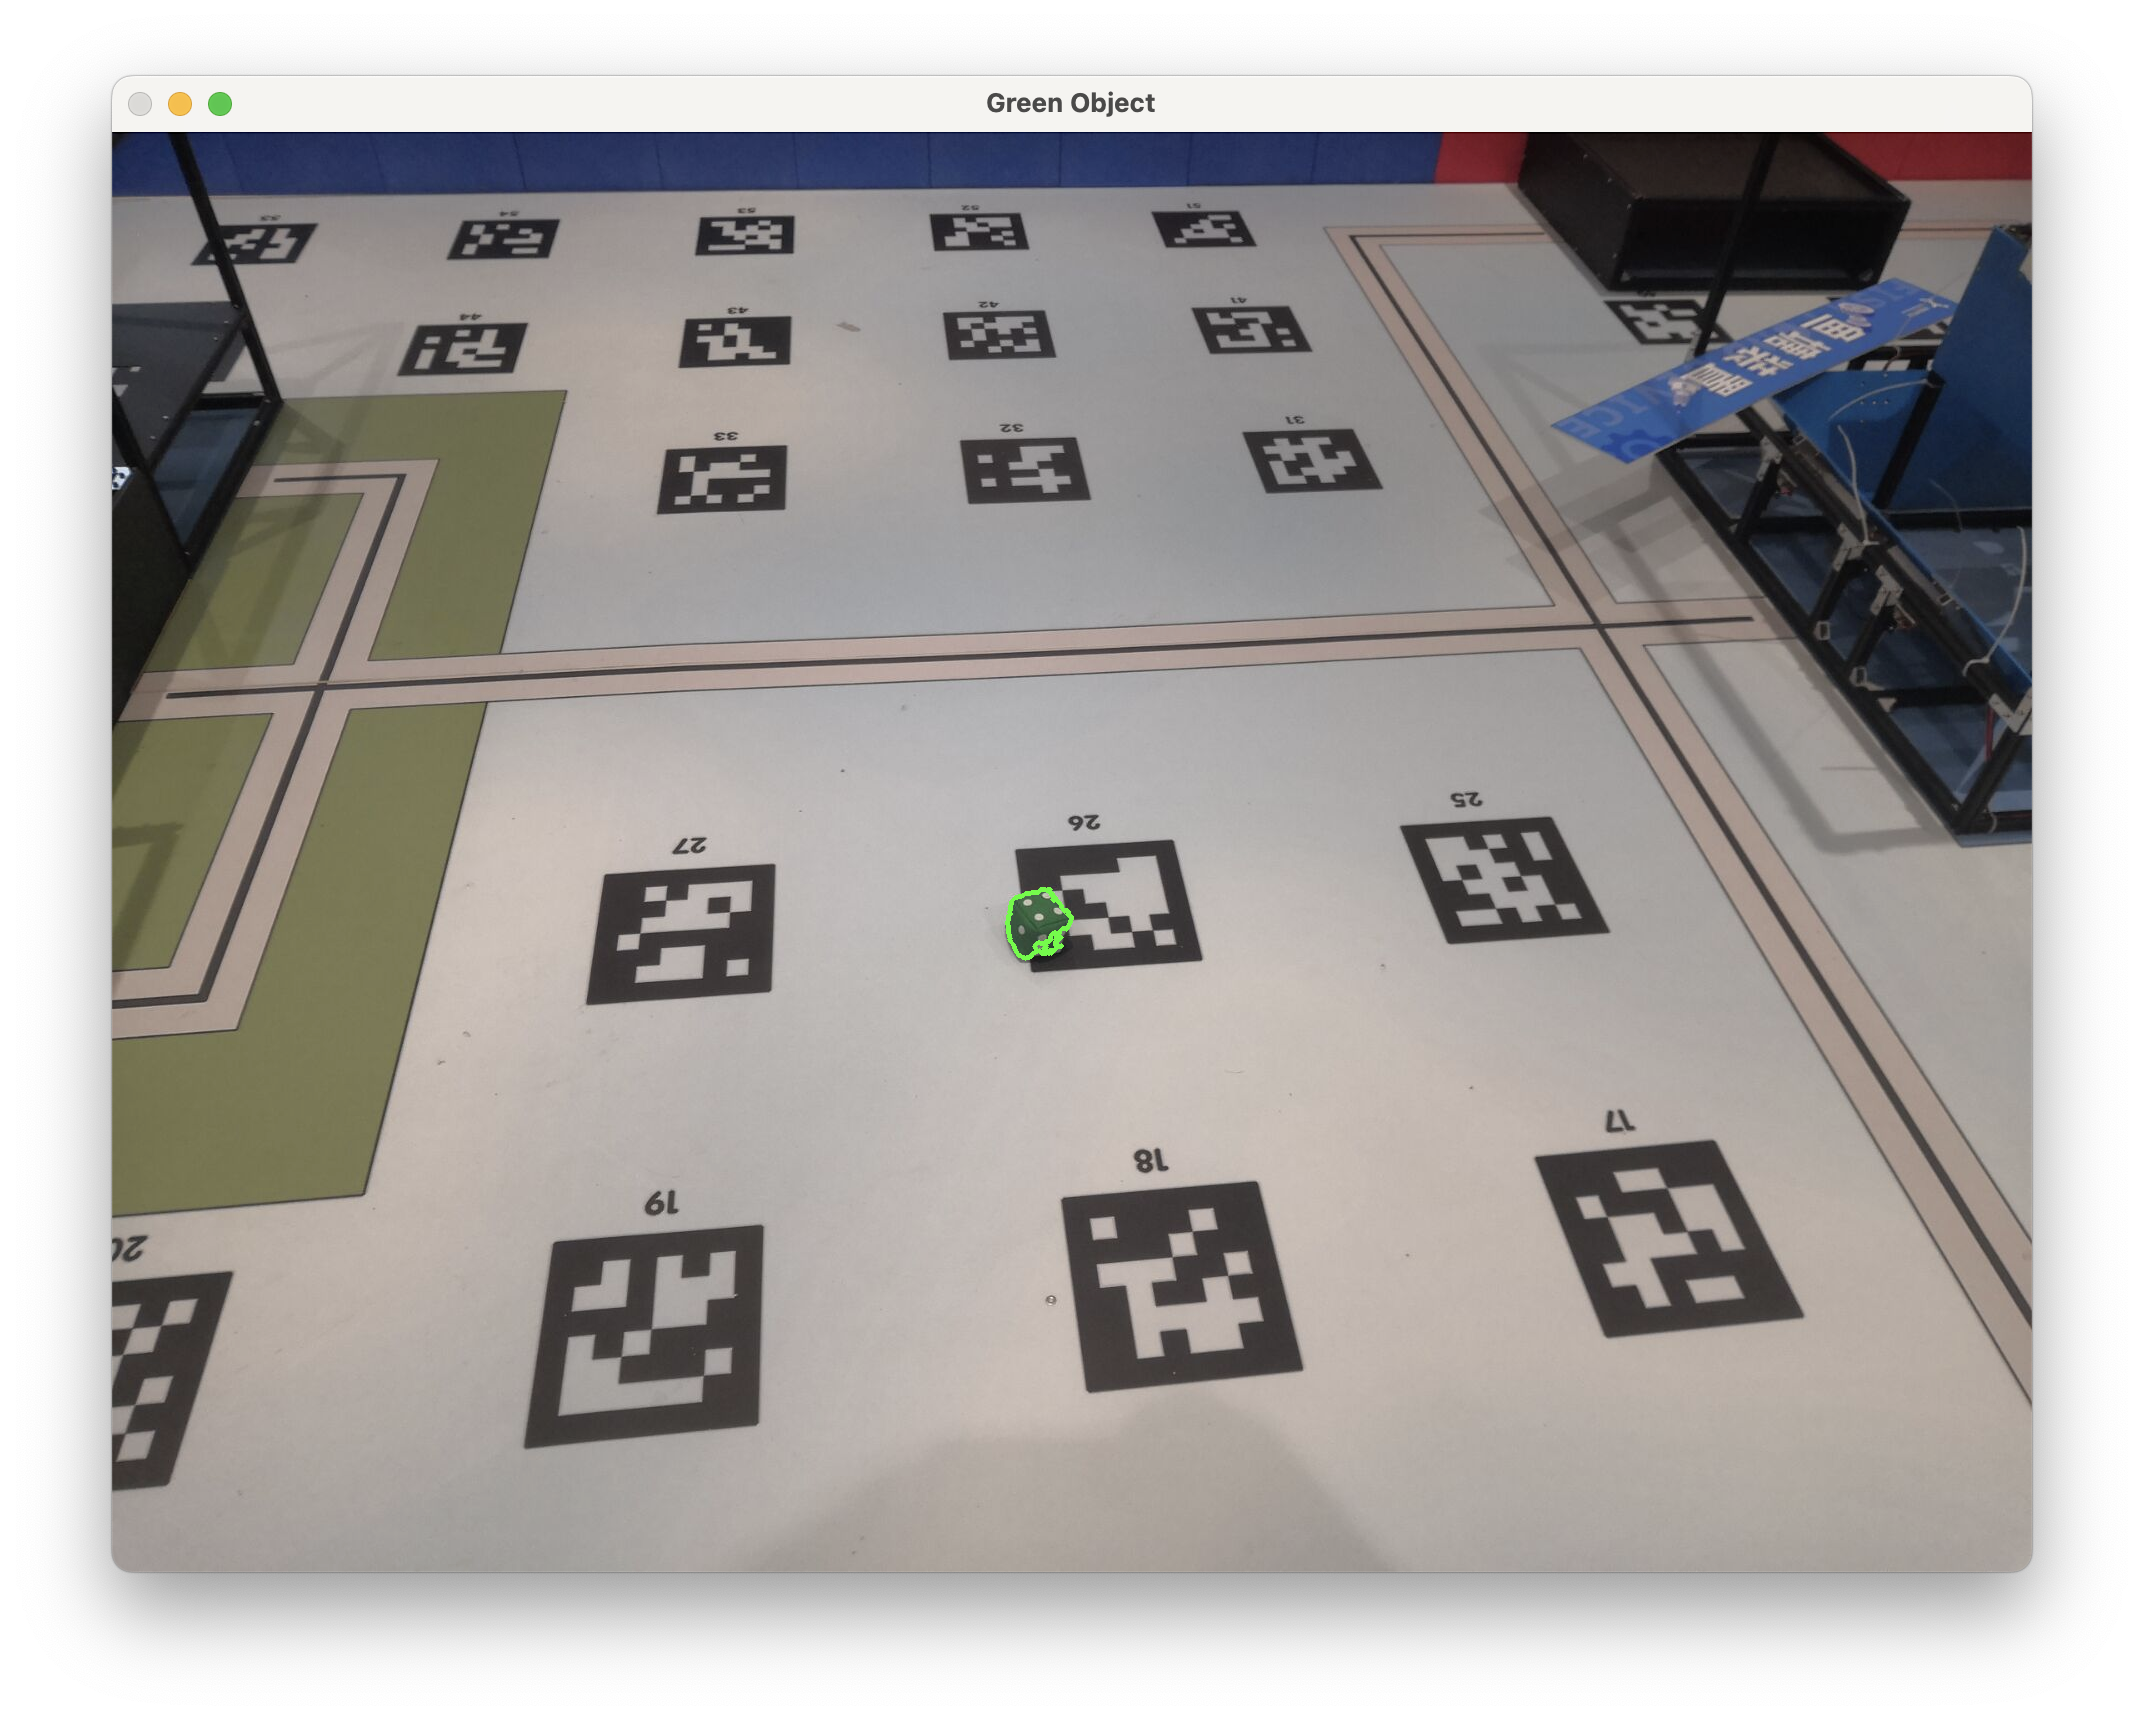
\includegraphics[width=0.8\textwidth]{figure/r-1.png}

Then, adding the mask can make the recognition more accurate. We can recognize the border and then calculate the position of the block.

\appendix


\section{Git Repository}

The project is stored in the \texttt{GitHub} repository. You can visit the repository through the link: \url{
    https://github.com/A3-SZInnoX-2024/localization.git
}

\end{document}
